\pagebreak
\section{Vehicle's Inertia Test} \label{app:inertiaTest}
\textbf{Name: Group 510}\\
\textbf{Date: 02/11 - 2015}

\subsection{Purpose}
The purpose of this test is to ensure the fact that the magnetometer is calibrated so that it can tell a correct position relative to the Earth's magnetic field when placed on the vehicle.

\subsection{Theory}


\begin{figure}[H]
  \centering
  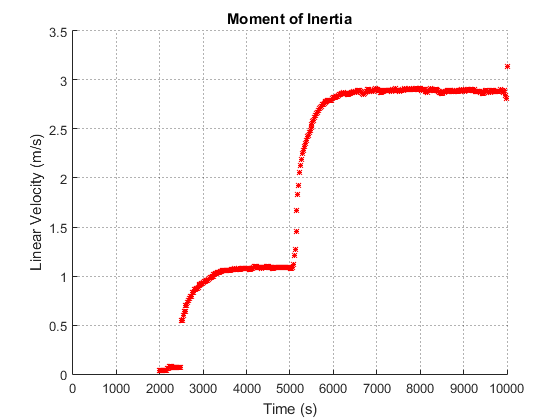
\includegraphics[scale=0.8]{figures/VehicleMomentOfInertiaTest.png}
  \caption{Vehicle's velocity response to a two-steps input}
  \label{fig:MomentOfInertiaTestPlot}
\end{figure}

%% Test setup description %%
\subsection{Setup}
\begin{figure}[H]
  \centering
  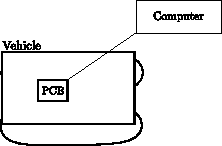
\includegraphics[scale=1.6]{figures/inertiaTestSetupDiagram2.pdf}
  \caption{Setup diagram}
  \label{inertiaTestSetupDiagram}
\end{figure}

\subsection{List of Equipment}

\begin{table}[H]
\begin{tabular}{|p{10cm}|p{4cm}|}
\hline%------------------------------------------------------------------------------------
  \textbf{Instrument}                     &  \textbf{Type}       \\
\hline%------------------------------------------------------------------------------------
  Computer                                &  Asus N73JN    \\
\hline %-----------------------------------------------------------------------------------
\end{tabular}
\end{table}

%% Procedure %%
\subsection{Procedure}

\begin{enumerate}
  \item Step 1
\end{enumerate}

%% Results %%
\subsection{Results} \label{inertiaTestResults}

